\section{Introduction à OpenCV}

\subsection{Lecture et affichage d'une image}

Pour cette introduction à OpenCV, nous allons d'abord commencer par voir comment récupérer
certaines informations d'une image. L'exemple suivant nous permet d'afficher dans l'ordre 
la définition, la taille en octets, la profondeur en bits et le nombre de canaux d'une image.\\

\begin{lstlisting}[caption=Afficher les champs de la structure IplImage]
  // Afficher des proprietes de l'image sur la console
  printf( "Infos sur l'image %s\n", nomImage.data() );
  // Definition (largeur x hauteur)
  printf( "Definition\t: %dx%d pixels\n", image->width, image->height );
  printf( "Taille \t\t: %d octets\n", image->imageSize );
  printf( "Profondeur \t: %d bits\n", image->depth );
  printf( "Nb de canaux \t: %d\n", image->nChannels );
  printf( "Appuyer sur une touche pour terminer.\n" );
\end{lstlisting}

%\begin{figure}[H]
%      \center
%      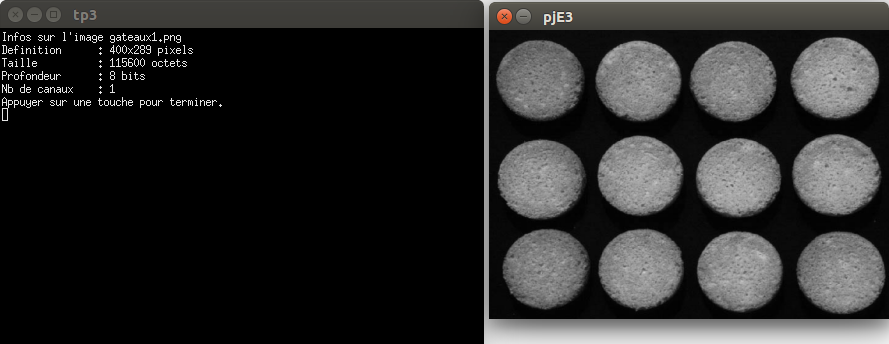
\includegraphics[width=16cm]{ressources/tp3/tp3_q1-1.png}
%      \caption{Résultat de l'affichage des champs de la structure IplImage sur la console}
%\end{figure}



Suite à l'affichage des quatre images, on peut voir que la taille dépend de la définition, du nombre 
de canaux et de la profondeur de l'image. En revanche, ces différents paramètres sont indépendants entre 
eux et leur variation n'est pas toujours visible directement sur l'image.\\

\begin{framed}
$$ 
 taille = largeur * hauteur * nb\_canaux * \frac{profondeur}{8}
$$
\\
{\footnotesize \textit{La profondeur est divisée par 8 pour passer d'un nombre en bits vers un nombre en octets.}}
\end{framed}

Lorsque l'on charge une image avec la fonction \textbf{cvLoadImage} d'OpenCV, il existe plusieurs 
modes de chargement, les plus fréquents sont : \\

\begin{itemize}
 \item \textbf{CV\_LOAD\_IMAGE\_UNCHANGED}, l'image est chargée avec les caractéristiques données lors 
de l'enregistrement de cette image. C'est-à-dire, si cette image a une profondeur de 16 bits alors 
elle aura une profondeur de 16 bits sous OpenCV.\\

 \item \textbf{CV\_LOAD\_IMAGE\_COLOR}, l'image est convertie vers une image de 24 bits par pixel, 3 canaux de 
8 bits, un canal pour chaque couleur (rouge, vert et bleu). Pour les images en niveau de gris, pour un pixel 
$x$ et $y$, les 3 canaux ont la même intensité que le pixel en $x$ et $y$ de l'image chargée. La valeur du canal en niveaux de gris est recopiée dans les canaux de chaque couleur.\\

 \item \textbf{CV\_LOAD\_IMAGE\_GRAYSCALE}, l'image est convertie vers une image de 8 bits par pixel, avec 
un canal, le niveau de gris. Lorsque l'image source est en couleur, le niveau de gris résultant est la 
somme des canaux rouge, vert et bleu auxquels on a appliqué un coefficient, en général de $\frac{1}{3}$.\\
\end{itemize}

\subsection{Transformations ponctuelles d'une image}

Afin d'analyser les variations de gris de l'image, nous avons affiché l'histogramme de celle-ci via 
l'outil Gimp.

\begin{figure}[H]
      \center
      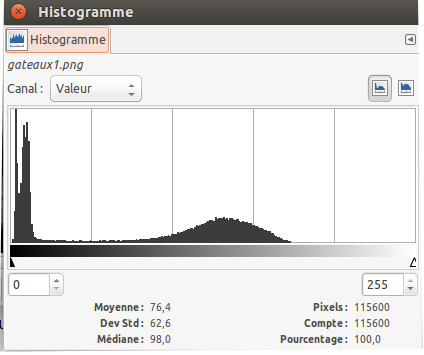
\includegraphics[width=8cm]{ressources/tp3/histogramme1.png}
      \caption{Histogramme de l'image gateau1.png vu avec l'outil Gimp}
\end{figure}

Ce graphique montre qu'il y a de nombreux pixels proches du noir (au début de l'histogramme) qui correspondent au fond de l'image.
Puis les pixels se concentrent dans une zone de gris qui représente les couleurs des gâteaux. À partir de ce graphique,
on peut déterminer approximativement la dynamique de l'image. La dynamique est la différence entre la plus grande valeur 
de niveau de gris de l'image et la plus petite. Sur l'histogramme que nous étudions, on peut voir que la dynamique est approximativement de 
177. Cette valeur ne correspond pas à la valeur que peut nous fournir la fonction \textbf{cvMinMaxLoc} qui est plus précise 
que ce que nous pouvons voir avec Gimp. Avec cette fonction, nous avons une dynamique de 201.\\

La binarisation va nous permettre de séparer clairement les gâteaux du fond. En utilisant l'outil Gimp, nous avons 
déterminé un seuil à 30 que l'on peut ensuite utiliser dans la fonction \textbf{cvThreshold}.\\

\begin{figure}[H]
      \center
      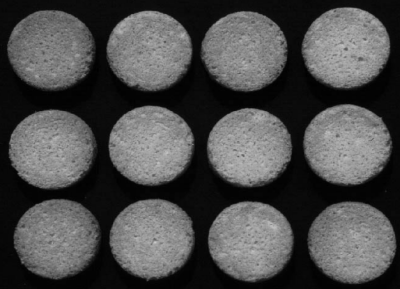
\includegraphics[width=5cm]{ressources/tp3/gateaux1.png}
      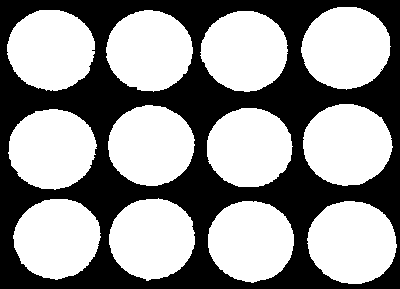
\includegraphics[width=5cm]{ressources/tp3/gateaux1_bin_gimp_T.png}
      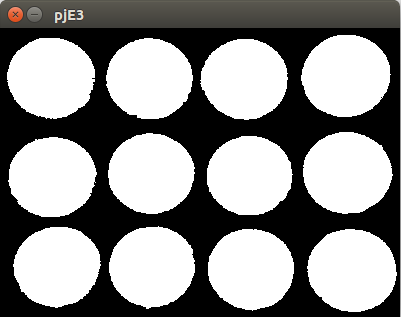
\includegraphics[width=5cm]{ressources/tp3/binarization_opencv.png}
      \caption{Binarisation des gâteaux. À gauche, l'image source. Au centre, seuillage à 30 avec gimp. À droit, idem avec OpenCV.}
\end{figure}

La fonction \textbf{cvCmp} d'OpenCV permet de comparer deux images, les pixels identiques entre les deux images sont représentés 
en noir. Nous allons utiliser une fonction pour comparer le seuillage d'OpenCV et de Gimp. La première fois avec un seuil à 30 sur 
OpenCV et Gimp, voir l'image de gauche ci-dessous. On note quelques différences entre les deux fonctions du fait des inclusions 
et exclusions des pixels qui ont la valeur du seuil. La seconde fois, la comparaison est effectuée avec un seuil à 30 sous OpenCV 
et un seuil à 60 (deux fois plus grand) avec Gimp, voir l'image de droite ci-dessous. La différence se trouve sur les bords des 
gâteaux. En effet, avec un seuil à 60, les bords des gateaux, qui sont plus sombre, sont considérés comme faisant partie du fond.\\

\begin{figure}[H]
      \center
      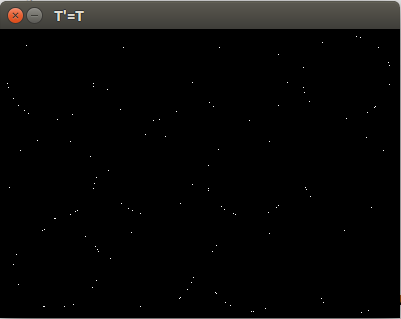
\includegraphics[width=5cm]{ressources/tp3/compare_T_T.png}
      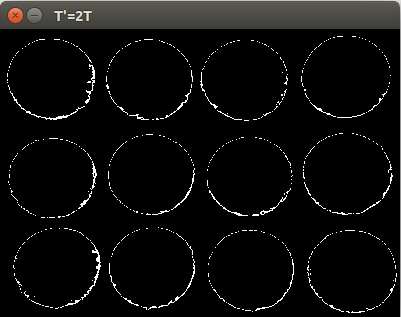
\includegraphics[width=5cm]{ressources/tp3/compare_T_2T.png}
      \caption{Comparaison des seuillages avec OpenCV et Gimp}
\end{figure}

Ensuite, l'utilisation de \textbf{cvThreshold} avec les flags \textbf{CV\_THRESH\_BINARY} et \\ \textbf{CV\_THRESH\_OTSU}, permet de binariser 
une image grâce à la méthode d'Otsu. Cette méthode détermine le seuil en prenant compte de l'histogramme. Ceci peut être pratique, mais ne 
donne pas toujours un meilleur résultat qu'avec un choix de seuil "à la main".

\begin{figure}[H]
      \center
      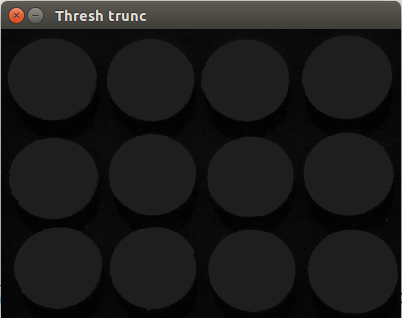
\includegraphics[width=5cm]{ressources/tp3/thresh_trunc.png}
      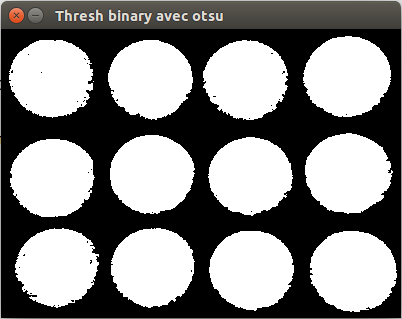
\includegraphics[width=5cm]{ressources/tp3/thresh_otsu.png}
      \caption{Autres méthodes de seuillage, CV\_TRUNC à gauche, CV\_BINARY avec Otsu à droite}
\end{figure}


\subsection{Parcours d'une image}

Avec OpenCV, les données d'une image sont changées dans la mémoire. L'adresse de début des données de l'image se trouve dans le 
pointeur d'octets \textbf{imageData} de la structure \textbf{IplImage}. C'est un vecteur unidimensionnel de valeurs des pixels. 
Les valeurs sont chargées de manière à ce que les lignes de l'image se suivent.\\

Exemple avec une image de de 3x3:\\

\begin{itemize}

  \item Valeurs des pixels dans l'image:
  \begin{tabular}{|c|c|c|}
    \hline
    10 & 24 & 156 \\
    \hline
    13 & 47 & 184 \\
    \hline
    28 & 95 & 230 \\
    \hline
  \end{tabular}\\
  
  \item Valeurs des pixels dans imageData:
  \begin{tabular}{|c|c|c|c|c|c|c|c|c|}
    \hline
    10 & 24 & 156 & 13 & 47 & 184 & 28 & 95 & 230 \\
    \hline
  \end{tabular}\\
 
\end{itemize}

Pour récupérer les valeurs de chaque pixel de l'image et appliquer un seuillage, il faut parcourir l'image de la manière suivante :

%\begin{lstlisting}[caption=Parcours d'une image avec OpenCV]
% int row, col;
% uchar niveau;

% for(col=0; col<image->height; col++) {
%   for(row=0; row<image->width; row++) {
%     niveau = (uchar)( image->imageData[ col*image->widthStep + row ] );
%   }
% }
%\end{lstlisting}

%\begin{lstlisting}[caption=Fonction getMax avec OpenCV]
%  uchar getMax(IplImage* image){
%  int row, col;
%  uchar max_val = 0;
%  uchar niveau;

%  for(col=0; col<image->height; col++){
%    for(row=0; row<image->width; row++){
%      niveau = (uchar)(image->imageData[col*image->widthStep + row]);
%      max_val = max(max_val, niveau);
%    }
%  }

%  return max_val;
%}
%\end{lstlisting}

\begin{lstlisting}[caption=Fonction seuiller avec OpenCV]
void seuiller(IplImage* imageSrc, IplImage* imageDst, uchar seuil){
  int row, col;
  uchar niveau;

  /* verification du format des images source et destination */
  if(imageSrc->imageSize!=imageDst->imageSize ||
     imageSrc->depth!=8 || imageDst->depth!=8 ||
     imageSrc->nChannels!=1 || imageDst->nChannels!=1){
       imageDst = NULL;
       return;
  }
  /* parcours des pixels de l'image source */
  for(col=0; col<imageSrc->height; col++){
    for(row=0; row<imageSrc->width; row++){
      niveau = (uchar)(imageSrc->imageData[ col*imageSrc->widthStep + row ]);

      /* application du seuil */
      if(niveau>seuil){
        imageDst->imageData[ col*imageDst->widthStep + row ] = 255;
      } else {
        imageDst->imageData[ col*imageDst->widthStep + row ] = 0;
      }
    }
  }
}
\end{lstlisting}
Le parcours d'une image couleur se fait un peu différemment du parcours d'une image en niveaux de gris.
En effet, la valeur des trois canaux se trouve à la suite dans le pointeur \textbf{imageData} d'\textbf{IplImage}.
Il faut donc avoir un pas de trois octets pour aller au pixel suivant. Les canaux sont rangés, par défaut, avec 
le bleu en premier puis le vert puis le rouge.\\

\begin{lstlisting}[caption=Fonction getCanal avec OpenCV]
void getCanal(IplImage* imageSrc, IplImage* imageDst, uchar canal){
  int row, col;

  // la position dans le tableau imageData
  // la position se caracterise par une ligne, une colonne et un canal
  int position;

  if(imageSrc->imageSize!=imageDst->imageSize ||
     imageSrc->depth!=8 || imageDst->depth!=8 ||
     imageSrc->nChannels!=3 || imageDst->nChannels!=3)
  {
    imageDst = NULL;
    return;
  }
  cvSet(imageDst, CV_RGB(0,0,0));

  for(col=0; col<imageSrc->height; col++){
    // Le pas est de 3 octets
    // La largeur de l'image est bien de imageSrc->width pixels, 
    // mais il y a 3 fois plus d'octets (les 3 canaux)
    for(row=0; row<imageSrc->width*3; row=row+3){
      position = col*imageSrc->widthStep + row + canal;
      imageDst->imageData[position] = imageSrc->imageData[position];
    }
  }
}
\end{lstlisting}
